\documentclass[border=10pt]{standalone}

\usepackage{tikz}
\usepackage{tikzsymbols}
\usetikzlibrary{calc,patterns,shapes.geometric}

\def\centerarc[#1](#2)(#3:#4:#5){\draw[#1] ($(#2)+({#5*cos(#3)},{#5*sin(#3)})$) arc (#3:#4:#5);}

\begin{document}
	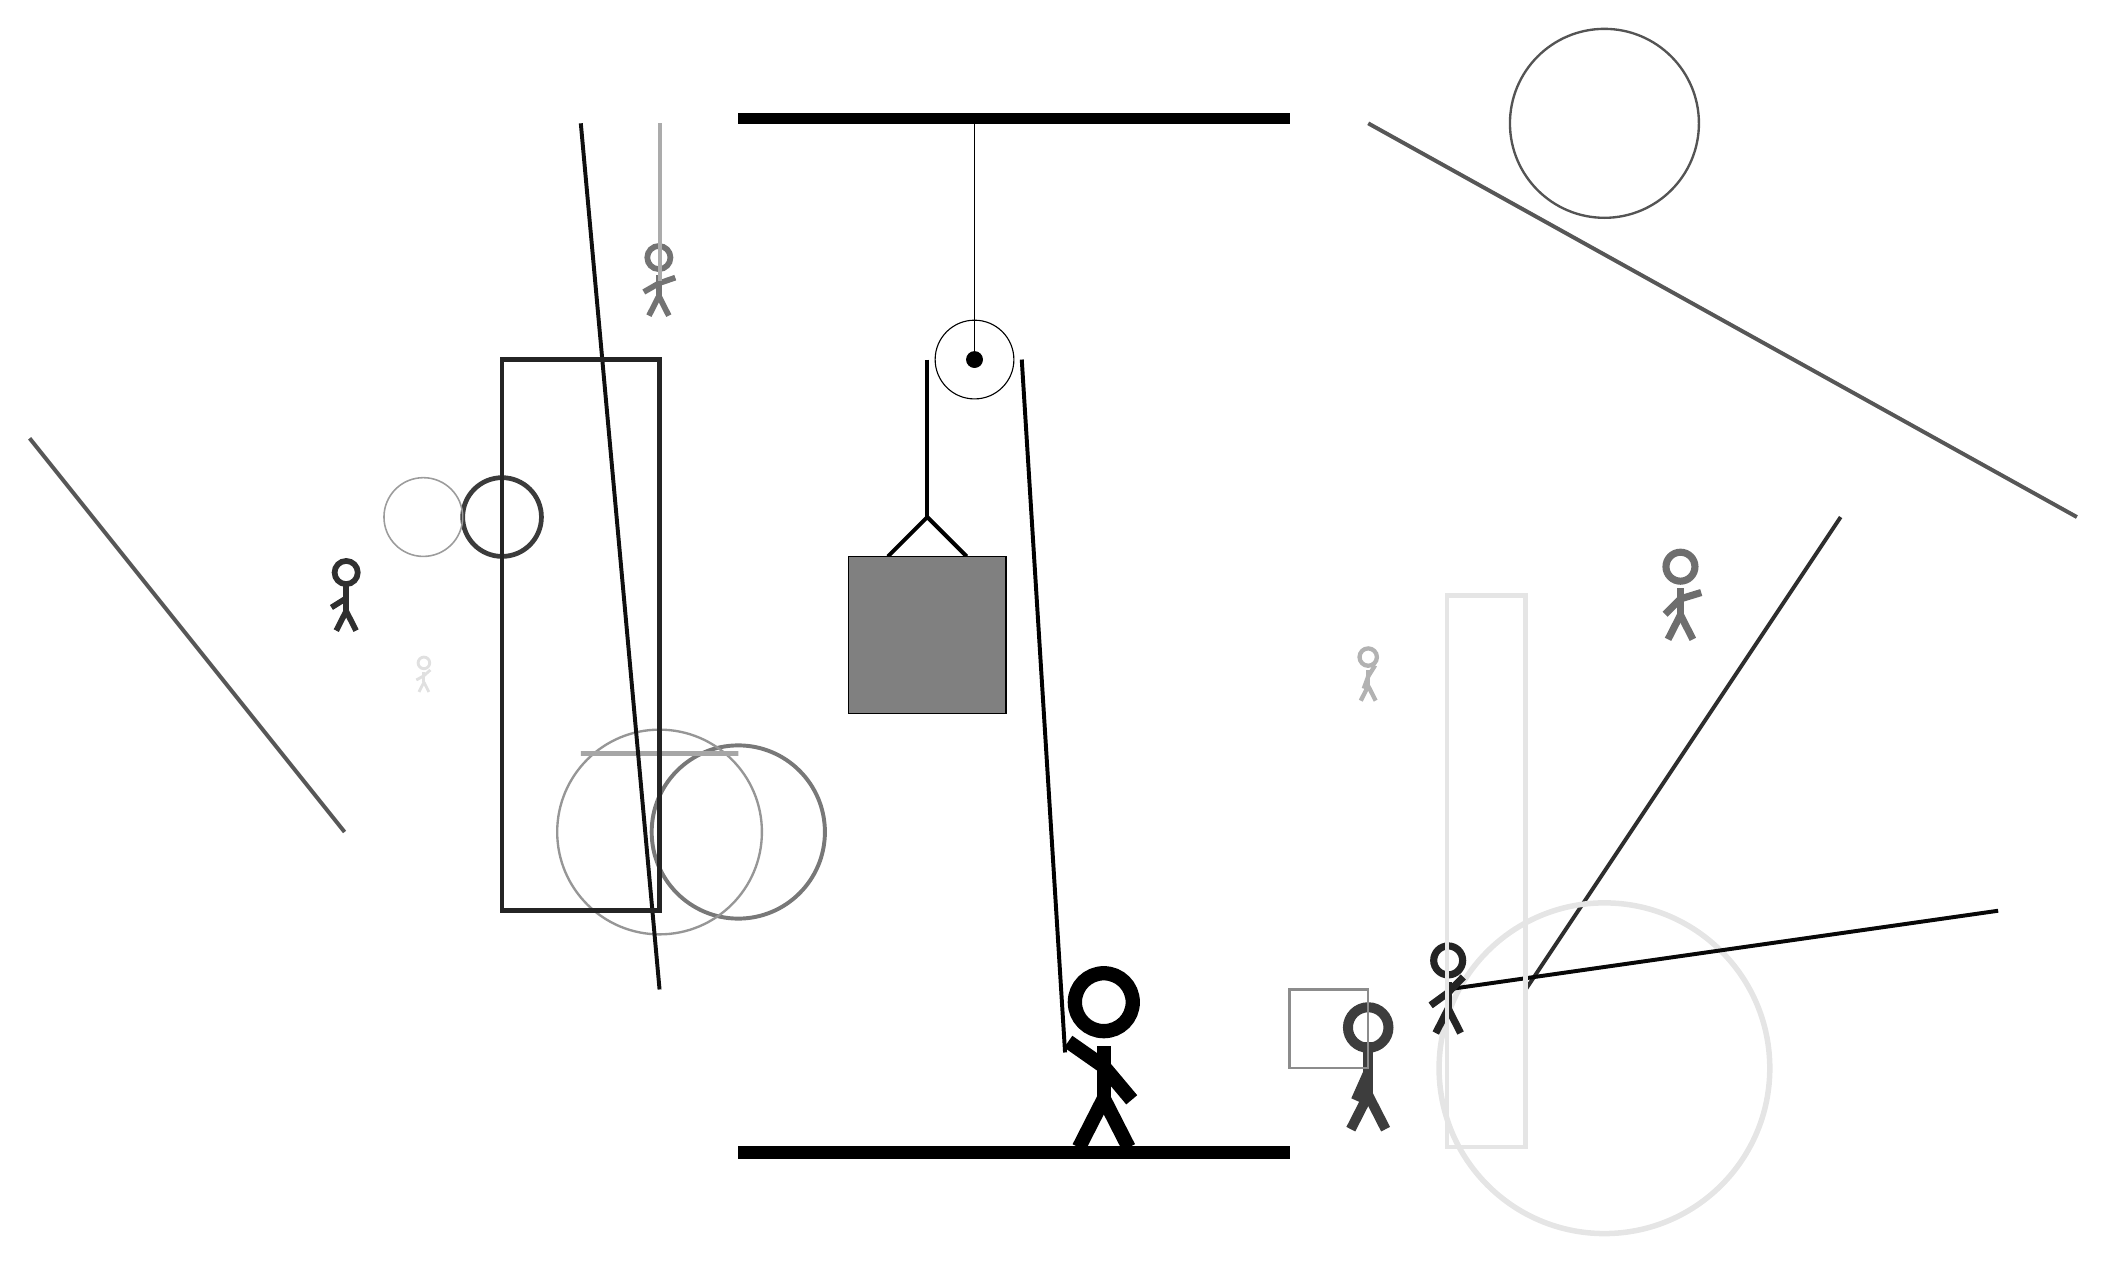
\begin{tikzpicture}
		%%%%% START %%%%%
		
		\draw[fill=black] (-2, 10) rectangle (5, 10.125);
		
		\draw (1, 7) circle (0.5);
		\draw[fill=black] (1, 7) circle (0.1);
		\draw (1, 10) -- (1, 7);
		
		\draw[line width=0.5mm] (-0.1, 4.5) -- (0.4, 5.0) -- (0.9, 4.5);
		\draw[fill=black!50] (-0.6, 4.5) rectangle (1.4, 2.5);
		
		\draw[line width=0.5mm, color=black!82](8, -1) -- (12, 5);
		
		\node[line width=0.6mm, color=black!57] at (10, 4) {\Strichmaxerl[5][45][17]};
		\draw [line width=0.7mm, color=black!10](9, -2) circle (2.1);
		\draw[line width=0.5mm, color=black!66](6, 10) -- (15, 5);
		\node[line width=0.2mm, color=black!12] at (-6, 3) {\Strichmaxerl[2][29][42]};
		\draw[line width=0.5mm, color=black!97](7, -1) -- (14, 0);
		
		\node[line width=0.2mm, color=black!76] at (6, -2) {\Strichmaxerl[7][66][90]};
		
		\node[line width=0.6mm, color=black!86] at (7, -1) {\Strichmaxerl[5][36][46]};
		\node[line width=0.7mm, color=black!55] at (-3, 8) {\Strichmaxerl[4][30][19]};
		
		\draw [line width=0.6mm, color=black!77](-5, 5) circle (0.5);
		\draw [line width=0.5mm, color=black!53](-2, 1) circle (1.1);
		\draw [line width=0.3mm, color=black!67](9, 10) circle (1.2);
		\node[line width=0.3mm, color=black!30] at (6, 3) {\Strichmaxerl[3][70][58]};
		\draw [line width=0.2mm, color=black!39](-6, 5) circle (0.5);
		\draw[line width=0.3mm, color=black!45] (5, -1) rectangle (6, -2);
		\draw [line width=0.3mm, color=black!41](-3, 1) circle (1.3);
		
		\draw[line width=0.5mm, color=black!66](-7, 1) -- (-11, 6);
		
		\draw[line width=0.6mm, color=black!10] (7, -3) rectangle (8, 4);
		\draw[line width=0.7mm, color=black!35] (-2, 2) rectangle (-4, 2);
		
		\draw[line width=0.5mm, color=black!94](-4, 10) -- (-3, -1);
		\node[line width=0.7mm, color=black!81] at (-7, 4) {\Strichmaxerl[4][32][90]};
		
		\draw[line width=0.6mm, color=black!86] (-3, 0) rectangle (-5, 7);
		\draw[line width=0.5mm, color=black!33](-3, 8) -- (-3, 10);
		
		\draw[line width=0.5mm] (0.4, 7) -- (0.4, 5.0);
		\centerarc[line width=0.5mm](1, 7)(0:180:0.6);
		\draw[line width=0.5mm](1.6, 7) -- (2.15, -1.8);
		
		\node at (2.6, -1.9) {\Strichmaxerl[10][-35][-50]};
		
		\draw[fill=black] (-2, -3) rectangle (5, -3.15);
		
		%%%%% END %%%%%
	\end{tikzpicture}
\end{document}